% Drawing 154/04-4 -- folder 154, batch 04, archive page 66 (PDF page 67).
% Transcription: figure : deux pseudo-droites orange se croisant sur une ligne de points noirs marquée $\delta$, un segment épais brun au point de croisement ; au-dessus, des hachures alternées vert clair et vert foncé, avec les orientations $\omega$ et « $\omega' = -\omega$ » en petites flèches courbes ; au-dessous, une courbe vert foncé en cloche fléchée à gauche ($\omega_{D'}$) et une droite vert clair fléchée à droite ($\omega_D$)
% Kind: two pseudolines crossing on a dotted line, alternating hatching, orientations. Method 2 (schematic redraw from the facsimile). Status: ok.
% Notes: Two orange pseudolines crossing on a line of black points (delta), a thick brown segment at the crossing; above, alternating light green and dark green hatching, with the orientations omega and « omega' = -omega » as small curved arrows (drawn as labels); below, a dark green bell-shaped curve arrowed to the left (omega_{D'}) and a light green line arrowed to the right (omega_D). Read from the page view; the small labels are placed, not all read.
% Coordinates: 1 unit = 1 mm = 1/100 of the crop width (bbox in page fractions: [0.601, 0.252, 0.864, 0.364]).
% Redrawn by Claude (claude-opus-5-5), issue #73, 2026-11-07; not checked by a human; not compiled (no TeX in the session).
% Revised by Claude (claude-opus-5-5) 2026-11-09 (issue #128) after Michel's check: vertices snapped to exact intersections (drawn points on their lines, meeting ends on the stroke they meet, near-concurrent lines through one computed point, curve ends on their rim); labels at \small as in folder 80 batch 3. Status: ok.
% Rights: reproduces part of the work -- behind RENDER_TRANSCRIPTS, never published by itself.
\documentclass[tikz,border=3pt]{standalone}
\usepackage{amsmath,amssymb}
\usetikzlibrary{patterns,arrows.meta}
\tikzset{Or/.style={orange!90!black}, Ye/.style={yellow!80!orange}, Lg/.style={green!60!black!70}, Dg/.style={green!45!black}, Br/.style={brown!80!black}, Rd/.style={red!85!black}, Bl/.style={blue!70!black}, Gy/.style={black!40}, pencil/.style={black!45}, struck/.style={black!35}, mark/.style={circle,draw,inner sep=1.3pt}, pt/.style={circle,fill,inner sep=0.9pt}, opt/.style={circle,draw,fill=white,inner sep=1.1pt}}
\colorlet{Or}{orange!90!black}\colorlet{Ye}{yellow!80!orange}\colorlet{Lg}{green!60!black!70}\colorlet{Dg}{green!45!black}\colorlet{Br}{brown!80!black}\colorlet{Rd}{red!85!black}\colorlet{Bl}{blue!70!black}\colorlet{Gy}{black!40}
\begin{document}
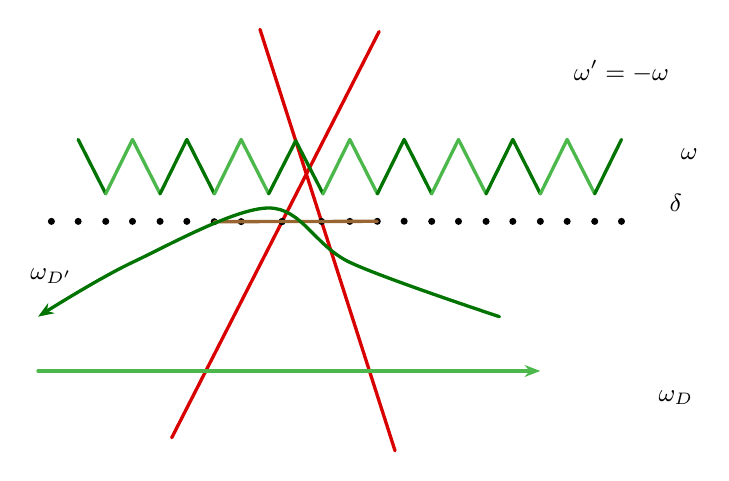
\begin{tikzpicture}[x=1mm,y=1mm,line cap=round,line join=round,font=\scriptsize]
\draw[Rd,very thick] (22.18,-55.08) -- (48.52,-3.49);
\draw[Rd,very thick] (33.39,-3.21) -- (50.54,-56.73);
\node[pt] at (6.9,-27.6) {};
\node[pt] at (10.3,-27.6) {};
\node[pt] at (13.8,-27.6) {};
\node[pt] at (17.2,-27.6) {};
\node[pt] at (20.7,-27.6) {};
\node[pt] at (24.1,-27.6) {};
\node[pt] at (27.58,-27.64) {};
\node[pt] at (31,-27.63) {};
\node[pt] at (36.2,-27.62) {};
\node[pt] at (36.2,-27.62) {};
\node[pt] at (41.21,-27.61) {};
\node[pt] at (44.8,-27.6) {};
\node[pt] at (48.29,-27.59) {};
\node[pt] at (51.7,-27.58) {};
\node[pt] at (55.2,-27.6) {};
\node[pt] at (58.6,-27.6) {};
\node[pt] at (62.1,-27.6) {};
\node[pt] at (65.5,-27.6) {};
\node[pt] at (69,-27.6) {};
\node[pt] at (72.4,-27.6) {};
\node[pt] at (75.9,-27.6) {};
\node[pt] at (79.3,-27.6) {};
\draw[Br,very thick] (27.58,-27.64) -- (48.29,-27.59);
\draw[Dg,very thick] (13.8,-24.1) -- (10.3,-17.2);
\draw[Lg,very thick] (20.7,-24.1) -- (17.2,-17.2);
\draw[Dg,very thick] (27.6,-24.1) -- (24.1,-17.2);
\draw[Lg,very thick] (34.5,-24.1) -- (31,-17.2);
\draw[Dg,very thick] (41.4,-24.1) -- (37.93,-17.36);
\draw[Lg,very thick] (48.3,-24.1) -- (44.8,-17.2);
\draw[Dg,very thick] (55.2,-24.1) -- (51.7,-17.2);
\draw[Lg,very thick] (62.1,-24.1) -- (58.6,-17.2);
\draw[Dg,very thick] (69,-24.1) -- (65.5,-17.2);
\draw[Lg,very thick] (75.9,-24.1) -- (72.4,-17.2);
\draw[Lg,very thick] (13.8,-24.1) -- (17.2,-17.2);
\draw[Dg,very thick] (20.7,-24.1) -- (24.1,-17.2);
\draw[Lg,very thick] (27.6,-24.1) -- (31,-17.2);
\draw[Dg,very thick] (34.5,-24.1) -- (37.93,-17.36);
\draw[Lg,very thick] (41.4,-24.1) -- (44.8,-17.2);
\draw[Dg,very thick] (48.3,-24.1) -- (51.7,-17.2);
\draw[Lg,very thick] (55.2,-24.1) -- (58.6,-17.2);
\draw[Dg,very thick] (62.1,-24.1) -- (65.5,-17.2);
\draw[Lg,very thick] (69,-24.1) -- (72.4,-17.2);
\draw[Dg,very thick] (75.9,-24.1) -- (79.3,-17.2);
\node[inner sep=1pt] at (87.9,-19) {\small $\omega$};
\node[inner sep=1pt] at (79.3,-8.6) {\small $\omega'=-\omega$};
\node[inner sep=1pt] at (86.2,-25.2) {\small $\delta$};
\draw[Dg,very thick,-{Stealth[length=2mm]}] plot[smooth, tension=0.55] coordinates {(63.8,-39.7) (44.8,-32.8) (34.5,-25.9) (17.2,-32.8) (5.2,-39.7)};
\node[inner sep=1pt] at (6.9,-34.5) {\small $\omega_{D'}$};
\draw[Lg,very thick,-{Stealth[length=2mm]}] (5.2,-46.6) -- (69,-46.6);
\node[inner sep=1pt] at (86.2,-50) {\small $\omega_D$};
\end{tikzpicture}
\end{document}
